\chapter{Visualización, evaluación de rendimiento y endurecimiento}
\label{cap:visualizacion}

El presente capítulo cierra la demostración del sistema con tres piezas.
Se recorren el panel de indicadores como resultado visible de toda la
plataforma, el banco de pruebas de rendimiento como evaluación
cuantitativa formal del procesamiento distribuido, y el endurecimiento
como evidencia de que el sistema se sometió a uso real y no solo a una
demostración controlada. El capítulo termina con la reconstrucción
completa de la plataforma desde cero, que cierra el objetivo de
reproducibilidad planteado en el Capítulo~\ref{cap:introduccion}.

\section{Panel de indicadores}
\label{sec:visualizacion_panel}

El panel se construye con Apache Superset~\cite{apache_superset_docs},
conectado a la base de datos PostgreSQL de la capa \textit{gold} descrita
en el Capítulo~\ref{cap:procesamiento}, nunca a Iceberg ni a Spark
directamente. La conexión usa un rol de solo lectura dedicado, distinto
del rol que publica los datos, con permiso de lectura sobre las tablas
existentes y sobre cualquier tabla futura del mismo esquema. Esa segunda
condición es necesaria porque la publicación de gold sustituye sus tablas
en cada ejecución del flujo, y un permiso otorgado solo sobre las tablas
actuales se perdería en la primera sustitución.

El panel muestra siempre agregados, nunca el nombre de una persona
concreta, aunque la tabla de dimensión de investigadores sí contiene
nombres reales tomados de ORCID. Ningún gráfico del panel consulta esa
tabla. El panel se define como código versionado, exportado a un paquete
reproducible en lugar de dejarse como configuración manual solo accesible
desde la interfaz. Esa exportación se verificó de forma directa. Tras
borrar por completo el panel, sus gráficos, sus conjuntos de datos y su
conexión, reimportar el paquete exportado reprodujo exactamente el mismo
panel, con el mismo identificador interno y con cada gráfico devolviendo
las mismas filas que antes del borrado.

El panel, mostrado en la Figura~\ref{fig:tfm_panel_superset}, reúne
cuatro elementos:

\begin{itemize}
  \item \textbf{Publicaciones por año.} El primer indicador de
  investigación, agregado por año de publicación.
  \item \textbf{Línea temporal de afiliaciones.} El tercer indicador,
  agregado por año de inicio y tipo de periodo.
  \item \textbf{Pares de colaboración.} El segundo indicador, restringido
  a los pares que involucran solo datos reales de ORCID, sin ningún
  miembro procedente de un CVN sintético.
  \item \textbf{Procedencia.} Una tabla con el identificador de la última
  ejecución del flujo de transformación y sus recuentos, para que cada
  cifra del panel pueda atribuirse a una ejecución concreta.
\end{itemize}

\begin{figure}[H]
  \centering
  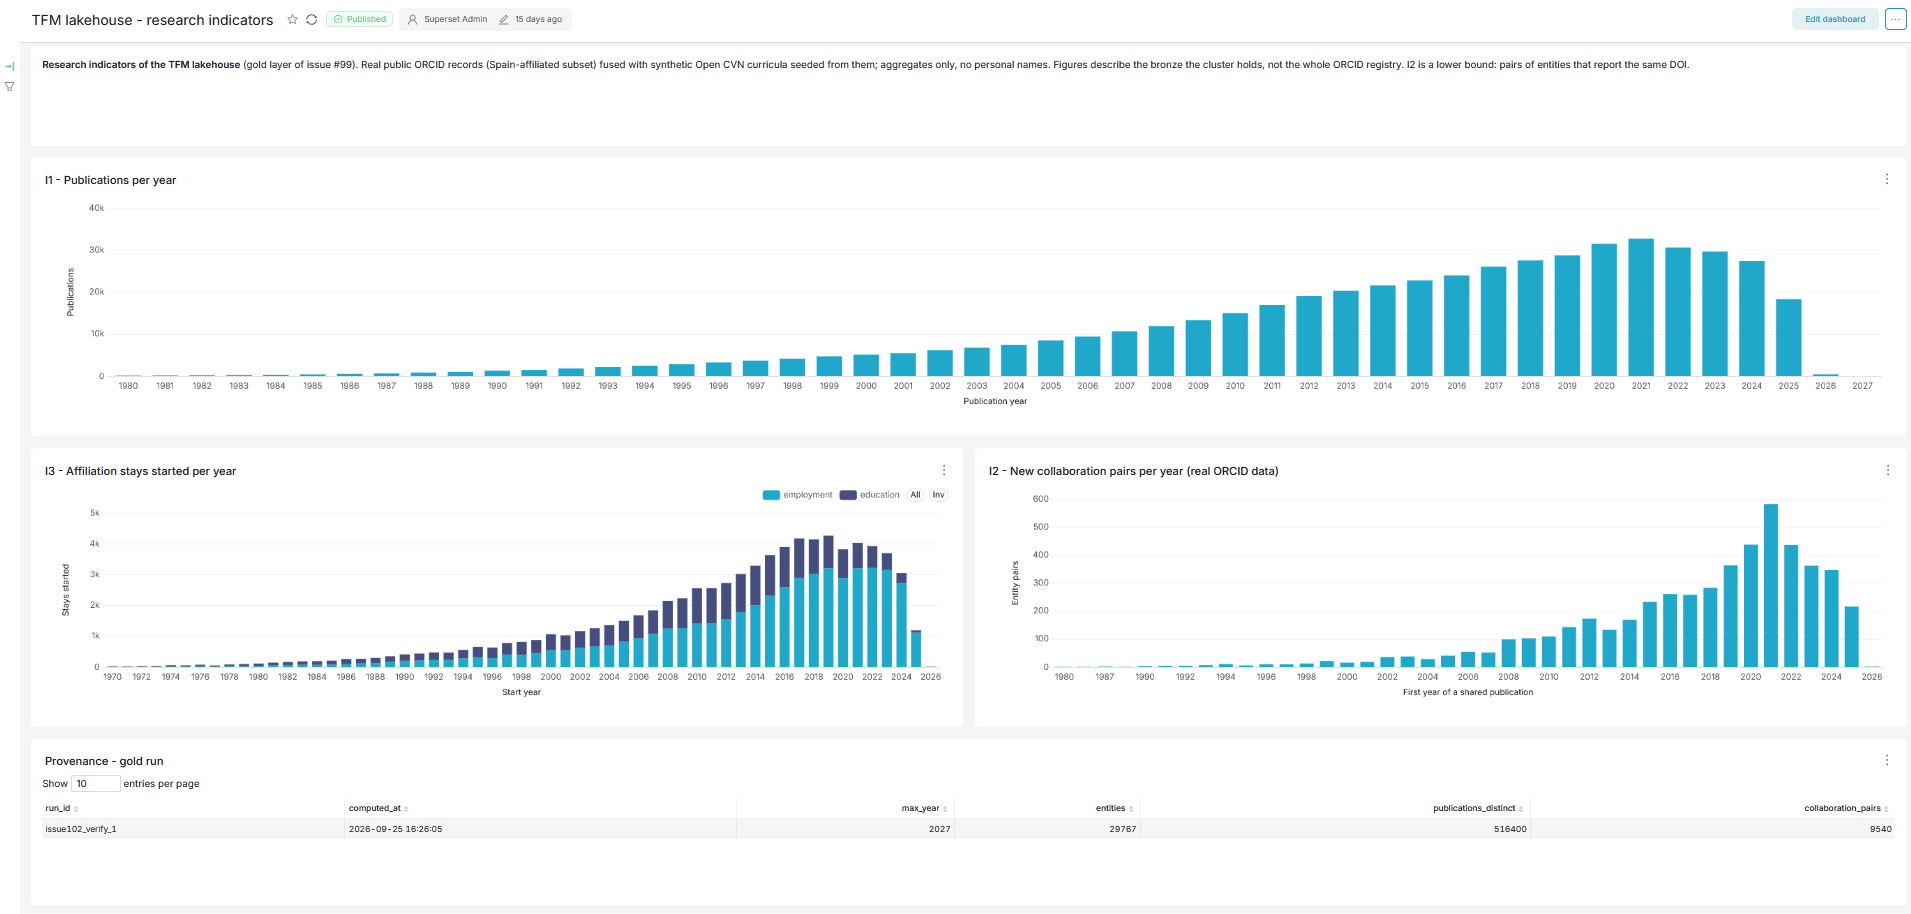
\includegraphics[width=\textwidth]{figs/panel_superset.png}
  \caption{Panel de indicadores de investigación en Apache Superset,
  con los tres indicadores y la tabla de procedencia de la ejecución.}
  \label{fig:tfm_panel_superset}
\end{figure}

La conexión del panel deshabilita además la caché de resultados, para que
una nueva ejecución del flujo de transformación se refleje de inmediato
sin necesidad de vaciarla a mano. Esto se verificó ejecutando el flujo de
transformación completo del Capítulo~\ref{cap:procesamiento} mientras un
proceso externo consultaba el panel de forma repetida. A lo largo de
1\,040 segundos y 238 consultas no se encontró ningún error ni ninguna
respuesta vacía. El identificador de ejecución mostrado por el panel pasó
de la ejecución anterior a la nueva en un único paso, sin ningún estado
intermedio visible, mientras el resto de cifras permanecía igual, como
corresponde a una transformación determinista sobre los mismos datos de
origen.

\section{Metodología y resultados del banco de pruebas de rendimiento}
\label{sec:visualizacion_benchmark}

El banco de pruebas mide el efecto del número de ejecutores de Spark sobre
el tiempo de los tres trabajos de transformación del
Capítulo~\ref{cap:procesamiento}, a tres escalas de volumen de datos y con
tres cantidades de ejecutores en cada una. La campaña se aísla por
completo de los datos de producción, con su propio cubo de MinIO, sus
propios espacios de nombres de Iceberg y su propio esquema de PostgreSQL
por escala, de forma que ninguna medición pueda alterar el panel del
Capítulo~\ref{cap:procesamiento} ni sus propios datos.

Cada combinación de escala y número de ejecutores se ejecuta varias veces.
La primera ejecución de cada escala se descarta como calentamiento, porque
leer un volumen de datos por primera vez resultó sistemáticamente más
lento que las ejecuciones siguientes. Las ejecuciones que sí cuentan se
repiten tres veces, intercaladas entre configuraciones en lugar de
agrupadas, para que una deriva del propio equipo durante la campaña no se
confunda con un efecto del número de ejecutores. La corrección de cada
resultado se comprueba además con una huella de contenido de las tablas
producidas, calculada de forma independiente de su orden. Dos
configuraciones distintas que terminan con éxito sobre la misma escala
deben producir exactamente la misma huella, y así ocurrió en todos los
casos comparables de la campaña.

La captura de estas métricas no necesitó desplegar una pila de
observabilidad dedicada como Prometheus~\cite{prometheus_docs} junto con
Grafana~\cite{grafana_docs}. Cada ejecución de Spark ya escribe su propio
registro de eventos, con la duración de cada etapa y tarea y el uso de
cada ejecutor, y ese registro basta para una campaña acotada como esta.
Instalar y operar una pila de observabilidad continua solo para esta
campaña puntual no estaba justificado, y queda documentada como trabajo
futuro para un despliegue en producción.

El hallazgo principal es que el número de ejecutores no es solo una
palanca de velocidad. A partir de cierto volumen, se convierte en una
palanca de fiabilidad. Con el dimensionamiento de memoria fijo por
ejecutor empleado en esta campaña, un único ejecutor deja de poder
completar el trabajo de validación y normalización de forma determinista
a partir del doble del volumen base, agotando su memoria en cada intento.
A cuádruple volumen, ni siquiera dos ejecutores bastan para ese mismo
trabajo, y solo se completa con cuatro. La Figura~\ref{fig:tfm_benchmark_silver}
muestra este comportamiento sobre el volumen base, donde el trabajo sí
completa a cualquier número de ejecutores.

\begin{figure}[H]
  \centering
  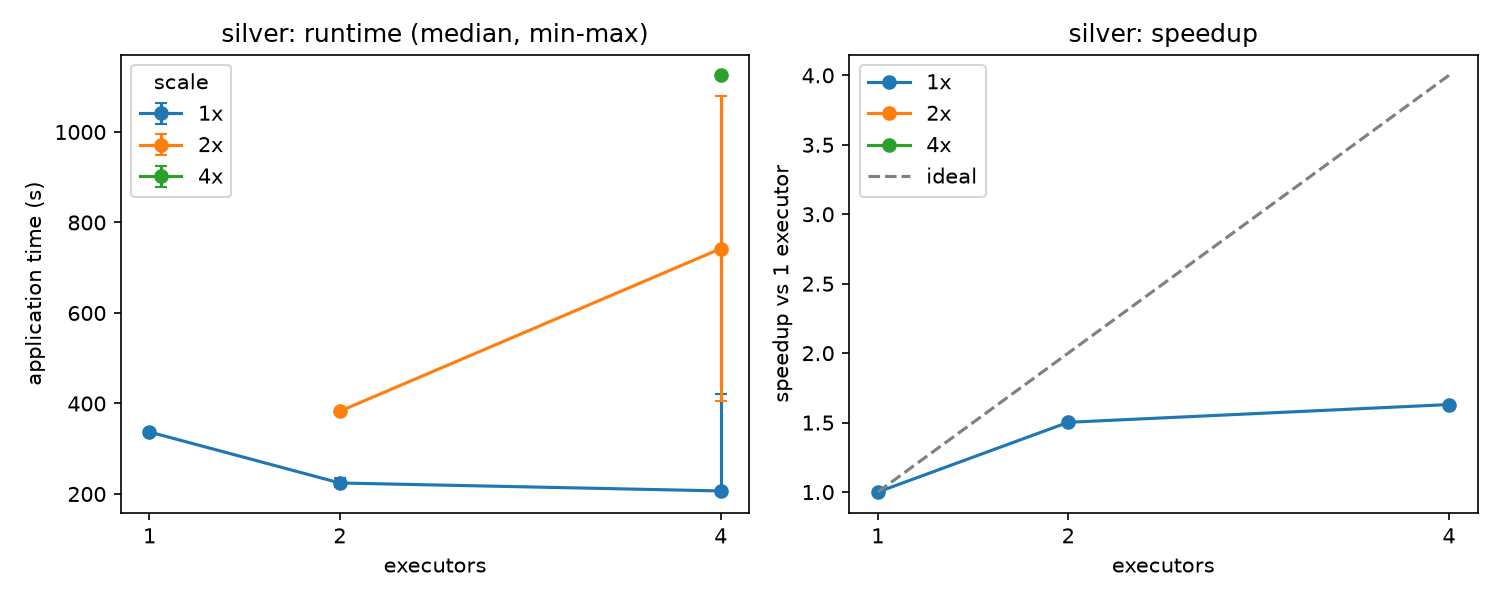
\includegraphics[width=\textwidth]{figs/benchmark_silver.png}
  \caption{Tiempo de ejecución y aceleración del trabajo de validación y
  normalización, sobre el volumen de datos base.}
  \label{fig:tfm_benchmark_silver}
\end{figure}

Incluso cuando el trabajo sí completa, la aceleración queda lejos de la
ideal. Sobre el volumen base, pasar de uno a dos ejecutores da una
aceleración de 1,50, y pasar a cuatro solo sube esa cifra a 1,63, con una
eficiencia que cae de 0,75 a 0,41. Los otros dos trabajos de la
transformación se comportan de forma todavía más marcada. El cálculo de
indicadores ve su eficiencia caer de 1,00 a 0,53 y a 0,23 al pasar de uno
a dos y a cuatro ejecutores, en cualquiera de las tres escalas, porque su
volumen de datos, ya agregado, es demasiado pequeño para aprovechar más
paralelismo. La publicación en PostgreSQL apenas crece con el volumen de
datos en absoluto, con un tiempo de entre 61 y 142 segundos en cualquier
combinación de escala y número de ejecutores, frente a un crecimiento
prácticamente lineal del trabajo de validación con el volumen. La
Tabla~\ref{tab:tfm_benchmark_exponentes} resume esta diferencia mediante
el exponente de la relación entre tiempo y volumen de datos, donde un
valor de 1 indica crecimiento lineal y un valor negativo indica que el
tiempo no depende del volumen.

\begin{table}[H]
  \centering
  \small
  \renewcommand{\arraystretch}{1.2}
  \begin{tabular}{
    >{\raggedright\arraybackslash}p{0.34\textwidth}
    p{0.18\textwidth} p{0.18\textwidth} p{0.18\textwidth}}
    \hline
    \textbf{Trabajo} & \textbf{1 ejecutor} & \textbf{2 ejecutores} & \textbf{4 ejecutores} \\
    \hline
    Validación y normalización & -- & 0,77 & 1,22 \\
    Cálculo de indicadores & 0,97 & 0,96 & 0,79 \\
    Publicación en PostgreSQL & -0,09 & -0,15 & -0,16 \\
    \hline
  \end{tabular}
  \caption{Exponente de crecimiento del tiempo de ejecución frente al
  volumen de datos, por trabajo y número de ejecutores.}
  \label{tab:tfm_benchmark_exponentes}
\end{table}

Ninguna de las tres etapas satura por falta de procesador. El uso de
sistema nunca superó el 32,2\% en ninguna ejecución, y ese máximo se dio
precisamente con cuatro ejecutores, el mismo punto donde el uso del
procesador del propio servicio de almacenamiento de objetos también
alcanzó su máximo. Este patrón apunta al almacenamiento de objetos
compartido, y no al procesador, como el límite más probable de la
plataforma en un único nodo. Esa lectura es consistente con los datos
disponibles, pero no queda demostrada de forma concluyente, ya que el
mecanismo exacto dentro del servicio de almacenamiento no se aisló más
allá de esta medición.

\section{Endurecimiento: fallos operativos reales encontrados y corregidos}
\label{sec:visualizacion_endurecimiento}

A diferencia de las limitaciones de diseño aceptadas de antemano en
capítulos anteriores, esta sección recoge fallos reales que aparecieron
usando el sistema completo bajo condiciones reales, no en una
demostración controlada. Encontrar y corregir un fallo de un componente
externo mediante diagnóstico y una recuperación operativa reproducible es,
en sí mismo, un resultado de este trabajo.

\begin{itemize}
  \item \textbf{Bloqueo permanente del orquestador de flujos.} Tras un
  periodo de funcionamiento sostenido, el propio servidor de tareas de
  Airflow quedó incapaz de arrancar, fallando de la misma forma en cada
  reinicio. La causa es un error conocido, sin corregir todavía en la
  versión de Airflow empleada, que se dispara al reconciliar una tarea
  huérfana cuyo pod ya no existe. El registro de esa tarea concreta
  quedaba almacenado sin marcarse como terminado, así que cada arranque
  del servidor volvía a intentar reconciliarla y volvía a fallar de la
  misma manera. Al tratarse de un error sin corrección disponible en la
  propia herramienta, la solución fue operativa en lugar de un cambio de
  código. Marcar manualmente esa tarea como fallida y reiniciar el
  servidor de tareas resolvió el bloqueo de inmediato. Esta misma
  incidencia volvió a producirse, de forma independiente, semanas
  después, y la misma receta operativa la resolvió de nuevo sin ningún
  cambio adicional.
  \item \textbf{Cierre del servidor de la interfaz de Airflow bajo carga.}
  Ese mismo servidor carecía de una reserva explícita de procesador y
  memoria, lo que le asignaba la prioridad de planificación más baja de
  todo el clúster. Bajo carga del propio nodo, quedaba desatendido el
  tiempo suficiente para que su propia comprobación de salud lo diera por
  bloqueado y lo reiniciase, interrumpiendo cualquier flujo que
  dependiera de él en ese momento. Se corrigió fijando una reserva
  explícita de recursos para ese servidor y relajando los tiempos de su
  comprobación de salud. La corrección se verificó en el propio clúster
  momentos después de que el fallo original volviera a producirse de
  forma independiente, confirmando que el nuevo ajuste resolvía
  exactamente ese mismo patrón.
\end{itemize}

\section{Verificación de extremo a extremo: reconstrucción desde cero}
\label{sec:visualizacion_verificacion}

La plataforma se diseñó para poder reconstruirse desde cero siguiendo
únicamente una guía escrita, sin pasos manuales no documentados. Esa guía
se validó en la práctica y no solo se redactó. La reconstrucción completa
se hizo sobre un clúster Kubernetes aislado y desechable, levantado con
k3d~\cite{k3d_docs}, en lugar de destruir el clúster real que ya contenía
los datos de producción de los capítulos anteriores. El clúster aislado
se configuró con la misma versión exacta de Kubernetes que el clúster
real, y con el propio repositorio de código montado en la misma ruta, de
forma que la guía se siguiera sin ningún paso distinto al que seguiría un
lector cualquiera.

Esta reconstrucción encontró un fallo real no observado hasta entonces.
Al arrancar todos los servicios base a la vez sobre un clúster
completamente nuevo, el primer arranque de PostgreSQL quedó interrumpido
por la contención de arrancar varios servicios a la vez, antes de llegar a
crear el usuario que la capa \textit{gold} necesita. La imagen empleada no
reintenta esa inicialización interrumpida en arranques posteriores, así
que el servicio quedaba disponible pero permanentemente incapaz de
autenticar ese usuario. El fallo se diagnosticó revisando el registro del
propio contenedor y se corrigió forzando una reinicialización completa de
ese servicio. Con esa corrección aplicada, la plataforma completa,
incluidos ambos flujos de Airflow y el panel de Superset con su propio
contenido importado, funcionó de extremo a extremo sobre el clúster
recién creado. El clúster aislado se eliminó al terminar, sin que el
clúster real ni sus datos de producción se vieran afectados en ningún
momento del proceso.
